
\documentclass[border=8pt, multi, tikz]{standalone} 
\usepackage{import}
\subimport{../layers/}{init}
\usetikzlibrary{positioning}
\usetikzlibrary{3d} %for including external image 


\def\ConvColor{rgb:yellow,5;red,2.5;white,5}
\def\ConvReluColor{rgb:yellow,5;red,5;white,5}
\def\PoolColor{rgb:red,1;black,0.3}
\def\UnpoolColor{rgb:blue,2;green,1;black,0.3}
\def\FcColor{rgb:blue,5;red,2.5;white,5}
\def\FcReluColor{rgb:blue,5;red,5;white,4}
\def\SoftmaxColor{rgb:magenta,5;black,7}   
\def\SumColor{rgb:blue,5;green,15}


\newcommand{\copymidarrow}{\tikz \draw[-Stealth,line width=0.8mm,draw={rgb:blue,4;red,1;green,1;black,3}] (-0.3,0) -- ++(0.3,0);}

\begin{document}
\begin{tikzpicture}
\tikzstyle{connection}=[ultra thick,every node/.style={sloped,allow upside down},draw=\edgecolor,opacity=0.7]
\tikzstyle{copyconnection}=[ultra thick,every node/.style={sloped,allow upside down},draw={rgb:blue,4;red,1;green,1;black,3},opacity=0.7]


\node[canvas is zy plane at x=0] (input) at (0,0,0) {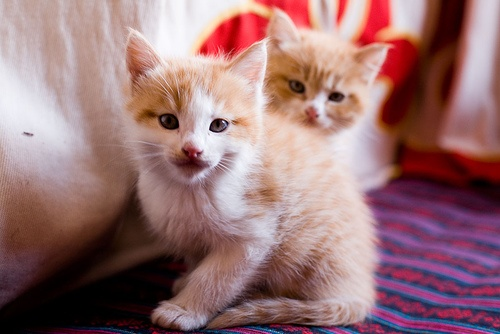
\includegraphics[width=8cm,height=8cm]{../examples/fcn8s/cats.jpg}};


\pic[shift={ (0,0,0) }] at (input-east) 
    {RightBandedBox={
        name=ccr_1,
        caption=Conv Block 1,
        xlabel={{ 64, 64 }},
        zlabel=256,
        fill=\ConvColor,
        bandfill=\ConvReluColor,
        height=40,
        width={ 2 , 2 },
        depth=40
        }
    };


\draw [connection]  (input-east)    -- node {\midarrow} (ccr_1-west);


\pic[shift={ (0,0,0) }] at (ccr_1-east) 
    {Box={
        name=pool_1,
        caption= ,
        fill=\PoolColor,
        opacity=0.5,
        height=32,
        width=1,
        depth=32
        }
    };


\draw [connection]  (ccr_1-east)    -- node {\midarrow} (pool_1-west);


\pic[shift={ (1,0,0) }] at (pool_1-east) 
    {RightBandedBox={
        name=ccr_2,
        caption=Conv Block 2,
        xlabel={{ 128, 128 }},
        zlabel=256,
        fill=\ConvColor,
        bandfill=\ConvReluColor,
        height=32,
        width={ 2 , 2 },
        depth=32
        }
    };


\draw [connection]  (pool_1-east)    -- node {\midarrow} (ccr_2-west);


\pic[shift={ (0,0,0) }] at (ccr_2-east) 
    {Box={
        name=pool_2,
        caption= ,
        fill=\PoolColor,
        opacity=0.5,
        height=24,
        width=1,
        depth=24
        }
    };


\draw [connection]  (ccr_2-east)    -- node {\midarrow} (pool_2-west);


\pic[shift={ (1,0,0) }] at (pool_2-east) 
    {RightBandedBox={
        name=ccr_3,
        caption=Conv Block 3,
        xlabel={{ 256, 256 }},
        zlabel=128,
        fill=\ConvColor,
        bandfill=\ConvReluColor,
        height=24,
        width={ 2 , 2 },
        depth=24
        }
    };


\draw [connection]  (pool_2-east)    -- node {\midarrow} (ccr_3-west);


\pic[shift={ (0,0,0) }] at (ccr_3-east) 
    {Box={
        name=pool_3,
        caption= ,
        fill=\PoolColor,
        opacity=0.5,
        height=16,
        width=1,
        depth=16
        }
    };


\draw [connection]  (ccr_3-east)    -- node {\midarrow} (pool_3-west);


\pic[shift={ (1,0,0) }] at (pool_3-east) 
    {RightBandedBox={
        name=ccr_bottleneck,
        caption=Bottleneck,
        xlabel={{ 512, 512 }},
        zlabel=64,
        fill=\ConvColor,
        bandfill=\ConvReluColor,
        height=16,
        width={ 4 , 4 },
        depth=16
        }
    };


\draw [connection]  (pool_3-east)    -- node {\midarrow} (ccr_bottleneck-west);


\pic[shift={ (2,0,0) }] at (ccr_bottleneck-east) 
    {Box={
        name=unpool_upconv_1,
        caption= ,
        fill=\UnpoolColor,
        opacity=0.5,
        height=16,
        width=1,
        depth=16
        }
    };


\pic[shift={ (0,0,0) }] at (unpool_upconv_1-east) 
    {RightBandedBox={
        name=ccr_res_upconv_1,
        caption= ,
        xlabel={{ 256, }},
        zlabel=64,
        fill={rgb:white,1;black,3},
        bandfill={rgb:white,1;black,2},
        opacity=0.5,
        height=16,
        width=5.0,
        depth=16
        }
    };


\pic[shift={(0,0,0)}] at (ccr_res_upconv_1-east) 
    {Box={
        name=ccr_upconv_1,
        caption= ,
        xlabel={{256, }},
        zlabel=64,
        fill=\ConvColor,
        height=16,
        width=5.0,
        depth=16
        }
    };


\pic[shift={ (0,0,0) }] at (ccr_upconv_1-east) 
    {RightBandedBox={
        name=ccr_res_c_upconv_1,
        caption= ,
        xlabel={{ 256, }},
        zlabel=64,
        fill={rgb:white,1;black,3},
        bandfill={rgb:white,1;black,2},
        opacity=0.5,
        height=16,
        width=5.0,
        depth=16
        }
    };


\pic[shift={(0,0,0)}] at (ccr_res_c_upconv_1-east) 
    {Box={
        name=upconv_1_out,
        caption= ,
        xlabel={{256, }},
        zlabel=64,
        fill=\ConvColor,
        height=16,
        width=5.0,
        depth=16
        }
    };


\draw [connection]  (ccr_bottleneck-east)    -- node {\midarrow} (unpool_upconv_1-west);


\path (ccr_3-southeast) -- (ccr_3-northeast) coordinate[pos=1.25] (ccr_3-top) ;
\path (ccr_res_upconv_1-south)  -- (ccr_res_upconv_1-north)  coordinate[pos=1.25] (ccr_res_upconv_1-top) ;
\draw [copyconnection]  (ccr_3-northeast)  
-- node {\copymidarrow}(ccr_3-top)
-- node {\copymidarrow}(ccr_res_upconv_1-top)
-- node {\copymidarrow} (ccr_res_upconv_1-north);


\pic[shift={ (2,0,0) }] at (upconv_1_out-east) 
    {Box={
        name=unpool_upconv_2,
        caption= ,
        fill=\UnpoolColor,
        opacity=0.5,
        height=24,
        width=1,
        depth=24
        }
    };


\pic[shift={ (0,0,0) }] at (unpool_upconv_2-east) 
    {RightBandedBox={
        name=ccr_res_upconv_2,
        caption= ,
        xlabel={{ 128, }},
        zlabel=128,
        fill={rgb:white,1;black,3},
        bandfill={rgb:white,1;black,2},
        opacity=0.5,
        height=24,
        width=4.5,
        depth=24
        }
    };


\pic[shift={(0,0,0)}] at (ccr_res_upconv_2-east) 
    {Box={
        name=ccr_upconv_2,
        caption= ,
        xlabel={{128, }},
        zlabel=128,
        fill=\ConvColor,
        height=24,
        width=4.5,
        depth=24
        }
    };


\pic[shift={ (0,0,0) }] at (ccr_upconv_2-east) 
    {RightBandedBox={
        name=ccr_res_c_upconv_2,
        caption= ,
        xlabel={{ 128, }},
        zlabel=128,
        fill={rgb:white,1;black,3},
        bandfill={rgb:white,1;black,2},
        opacity=0.5,
        height=24,
        width=4.5,
        depth=24
        }
    };


\pic[shift={(0,0,0)}] at (ccr_res_c_upconv_2-east) 
    {Box={
        name=upconv_2_out,
        caption= ,
        xlabel={{128, }},
        zlabel=128,
        fill=\ConvColor,
        height=24,
        width=4.5,
        depth=24
        }
    };


\draw [connection]  (upconv_1_out-east)    -- node {\midarrow} (unpool_upconv_2-west);


\path (ccr_2-southeast) -- (ccr_2-northeast) coordinate[pos=1.25] (ccr_2-top) ;
\path (ccr_res_upconv_2-south)  -- (ccr_res_upconv_2-north)  coordinate[pos=1.25] (ccr_res_upconv_2-top) ;
\draw [copyconnection]  (ccr_2-northeast)  
-- node {\copymidarrow}(ccr_2-top)
-- node {\copymidarrow}(ccr_res_upconv_2-top)
-- node {\copymidarrow} (ccr_res_upconv_2-north);


\pic[shift={ (2,0,0) }] at (upconv_2_out-east) 
    {Box={
        name=unpool_upconv_3,
        caption= ,
        fill=\UnpoolColor,
        opacity=0.5,
        height=32,
        width=1,
        depth=32
        }
    };


\pic[shift={ (0,0,0) }] at (unpool_upconv_3-east) 
    {RightBandedBox={
        name=ccr_res_upconv_3,
        caption= ,
        xlabel={{ 64, }},
        zlabel=256,
        fill={rgb:white,1;black,3},
        bandfill={rgb:white,1;black,2},
        opacity=0.5,
        height=32,
        width=3.5,
        depth=32
        }
    };


\pic[shift={(0,0,0)}] at (ccr_res_upconv_3-east) 
    {Box={
        name=ccr_upconv_3,
        caption= ,
        xlabel={{64, }},
        zlabel=256,
        fill=\ConvColor,
        height=32,
        width=3.5,
        depth=32
        }
    };


\pic[shift={ (0,0,0) }] at (ccr_upconv_3-east) 
    {RightBandedBox={
        name=ccr_res_c_upconv_3,
        caption= ,
        xlabel={{ 64, }},
        zlabel=256,
        fill={rgb:white,1;black,3},
        bandfill={rgb:white,1;black,2},
        opacity=0.5,
        height=32,
        width=3.5,
        depth=32
        }
    };


\pic[shift={(0,0,0)}] at (ccr_res_c_upconv_3-east) 
    {Box={
        name=upconv_3_out,
        caption= ,
        xlabel={{64, }},
        zlabel=256,
        fill=\ConvColor,
        height=32,
        width=3.5,
        depth=32
        }
    };


\draw [connection]  (upconv_2_out-east)    -- node {\midarrow} (unpool_upconv_3-west);


\path (ccr_1-southeast) -- (ccr_1-northeast) coordinate[pos=1.25] (ccr_1-top) ;
\path (ccr_res_upconv_3-south)  -- (ccr_res_upconv_3-north)  coordinate[pos=1.25] (ccr_res_upconv_3-top) ;
\draw [copyconnection]  (ccr_1-northeast)  
-- node {\copymidarrow}(ccr_1-top)
-- node {\copymidarrow}(ccr_res_upconv_3-top)
-- node {\copymidarrow} (ccr_res_upconv_3-north);


\pic[shift={(0.75,0,0)}] at (upconv_3_out-east) 
    {Box={
        name=softmax,
        caption=Softmax,
        zlabel=512,
        fill=\SoftmaxColor,
        height=40,
        width=1,
        depth=40
        }
    };


\draw [connection]  (upconv_3_out-east)    -- node {\midarrow} (softmax-west);


\end{tikzpicture}
\end{document}

